\documentclass[10pt]{beamer}


\usepackage[utf8]{inputenc}
\usetheme{metropolis}
\usepackage{appendixnumberbeamer}
\usepackage[defaultsans]{droidsans}

\usepackage{wrapfig}
\usepackage{tikz}
\usetikzlibrary{positioning}
\usepackage{fancyvrb}
\usepackage{booktabs}
\usepackage[scale=2]{ccicons}

\usepackage{xparse}

\usepackage{xspace}
\newcommand{\themename}{\textbf{\textsc{metropolis}}\xspace}

\usepackage{array}


\title{Mahalanobis-average \\Hierarchical Clustering Analysis \\accelerated on GPU}
%\subtitle{Defence}
\author{Bc. Adam Šmelko}
\date{Supervisor: RNDr. Miroslav Kratochvíl}
\institute{Department of Software Engineering}
\titlegraphic{\hfill
\includegraphics[height=2cm]{img/logo}}

\begin{document}

\maketitle


\begin{frame}{Mahalanobis distance}
	
	Measures a distance between a point and a distribution of points.
	
	\begin{figure}
		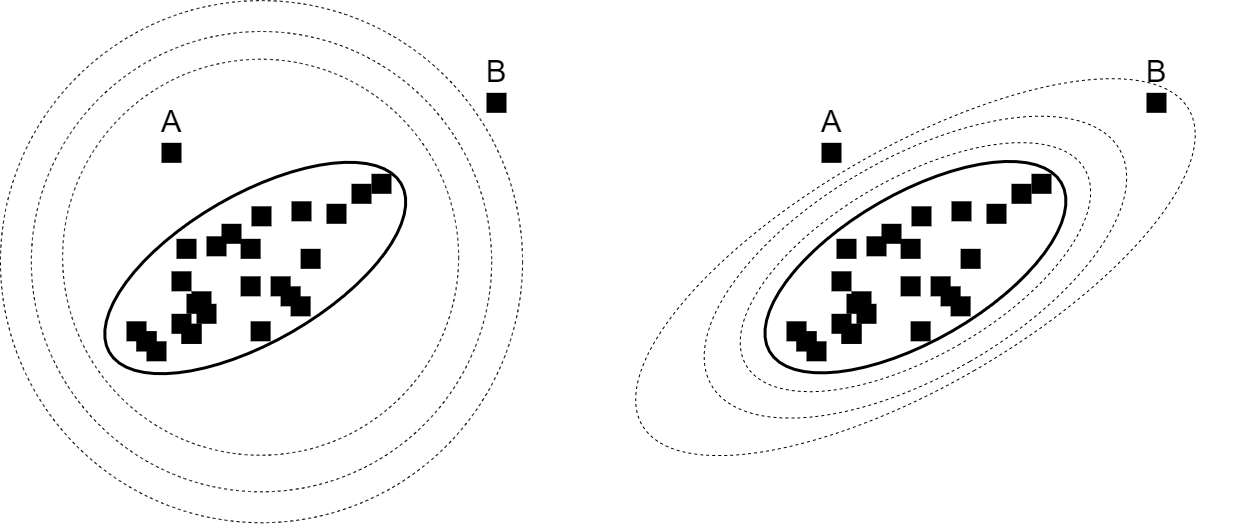
\includegraphics[width=7cm]{img/maha_dist}
	\end{figure}

	Computes the covariance matrix of a distribution which re-scales the axes.
		
\end{frame}


\begin{frame}{Mahalanobis-average clustering}
	
	Originally developed by Fišer et al. for the purpose of monitoring
	minimal residual disease in patients with leukemia.
	
	Naturally forms elliptic clusters.
	
	\begin{figure}
		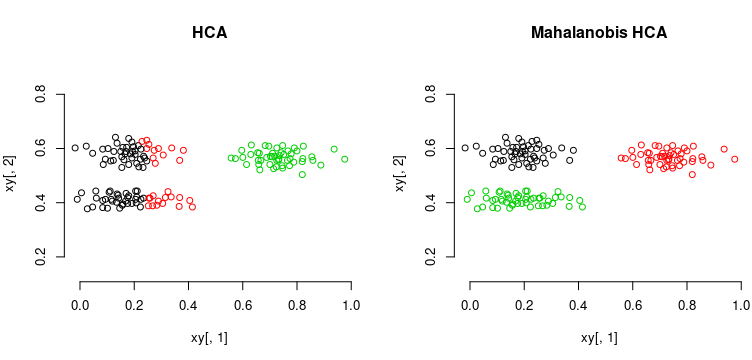
\includegraphics[width=7cm]{img/mhca}
	\end{figure}
	
	Extremely suitable for single-cell cytometry datasets.
	
\end{frame}

\begin{frame}{Motivation}

	Seriously restricted by performance and complexity to \textbf{$\pm$100K} cells on a common HW
	
	Modern cytometers produce \textbf{millions} \dots
	
	\begin{figure}
	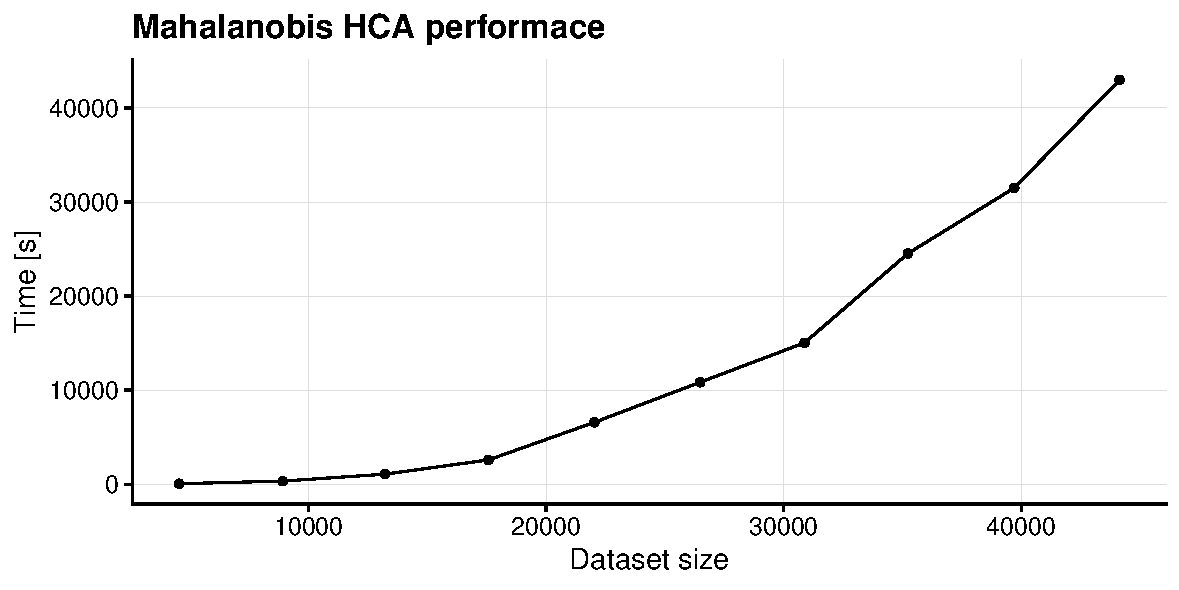
\includegraphics[width=8cm]{img/scalability}
	\end{figure}

\end{frame}

\begin{frame}{Challenges}
	
	Design an implementation with respect to:
	\begin{itemize}
		\item \emph{Performance}
		
		Solved by utilizing computing power of a GPU device.
		\item \emph{Huge input size}
		
		Polynomial space complexity is sub-optimal because the algorithm needs to cluster millions of points.
	\end{itemize}
	
\end{frame}

\begin{frame}{Results summary}
	
	Performance increase:
	\begin{itemize}
		\item 60 to 5000 times for single-point datasets
		\item 8 to 20 times for apriori datasets
	\end{itemize}

	Reduction of quadratic space complexity to linear.
	
	\textbf{Test machine}: Intel Xeon Silver 4110, 256 GB
	RAM, NVIDIA Tesla V100 PCIe 16 GB
	
\end{frame}

\begin{frame}{Results summary}
	
	\begin{tabular}{cc}
		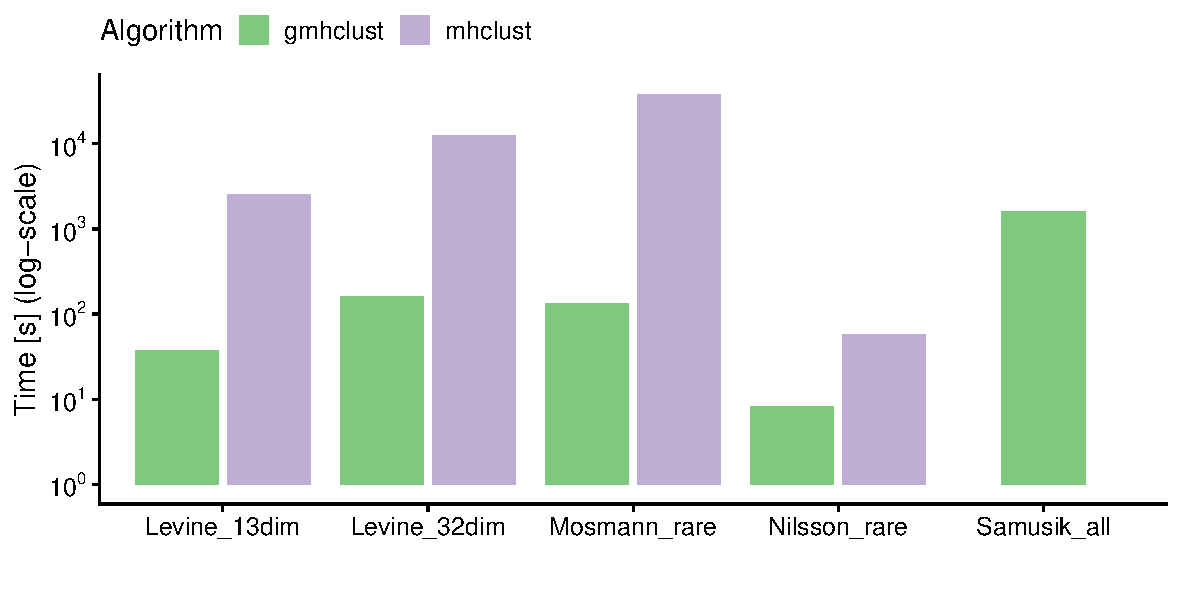
\includegraphics[width=6cm]{../img/mixed_perf_comp} & 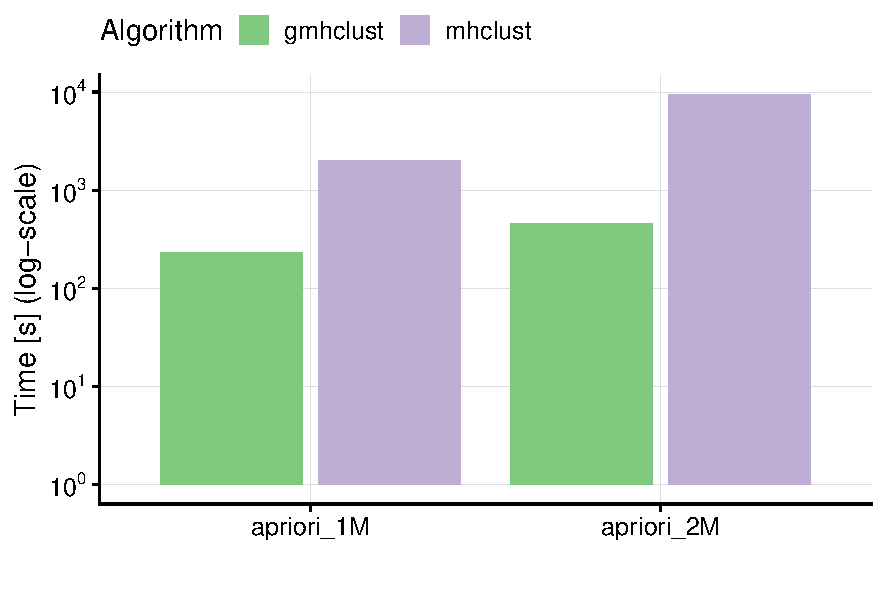
\includegraphics[width=4.4cm]{../img/apriori_perf_comp} \\
	\end{tabular}
	\begin{figure}
		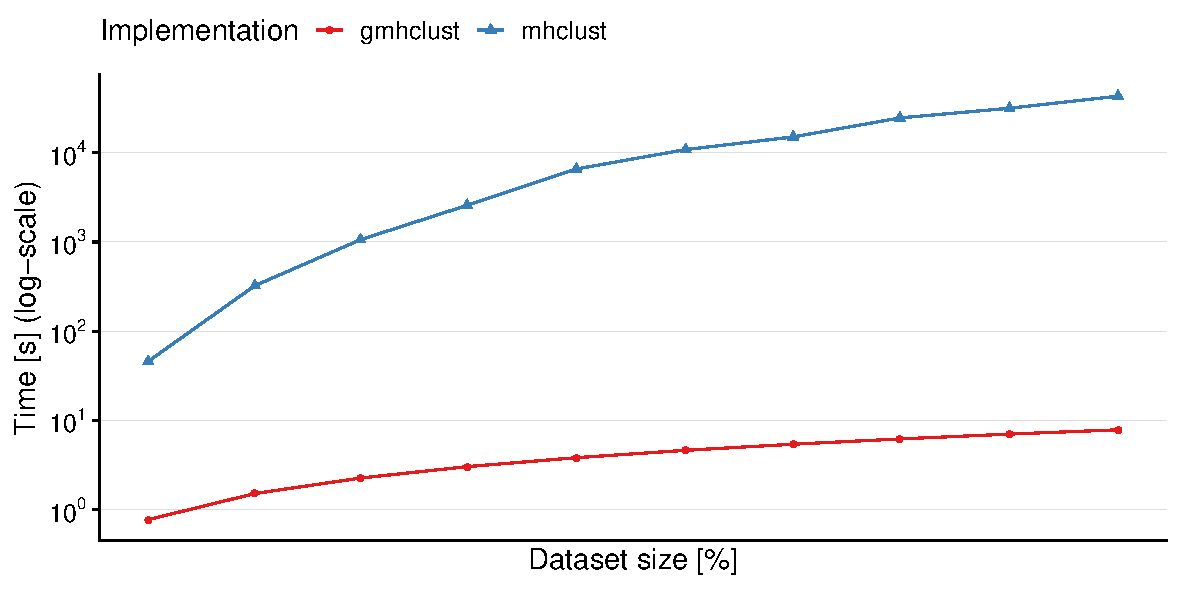
\includegraphics[width=7cm]{../img/single_perf_comp}
	\end{figure}
	
\end{frame}


\begin{frame}{Implementation details}
	
	The main principles:
	\begin{itemize}
		\item Data continuity
		\begin{figure}
			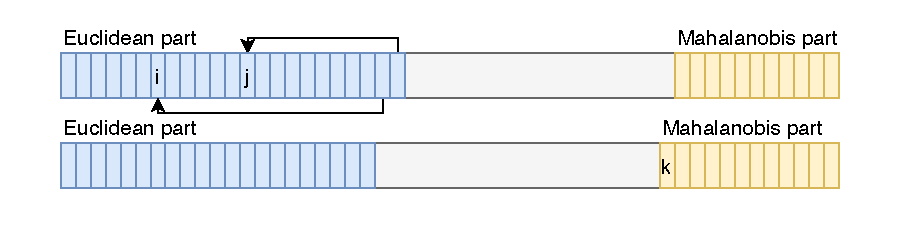
\includegraphics[width=8cm]{../img/data}
		\end{figure}
		
		\item Task-specific CUDA kernels
		\begin{itemize}
			\item \texttt{update\_eucl}
			\item \texttt{update\_maha}
			\item \texttt{compute\_centroid}
			\item \dots
		\end{itemize}
	\end{itemize}

\end{frame}

\begin{frame}{Implementation details}
	
	Used HCA variant: \textbf{Nearest neighbor HCA}
	\begin{itemize}
		\item Promises cubic time complexity (with possible enhancements) using linear space.
	\end{itemize}
	
	Future work:
	\begin{itemize}
		\item Switch to \textbf{Dissimilarity matrix HCA} when dataset is clustered to small size.
	\end{itemize}


	\begin{figure}
		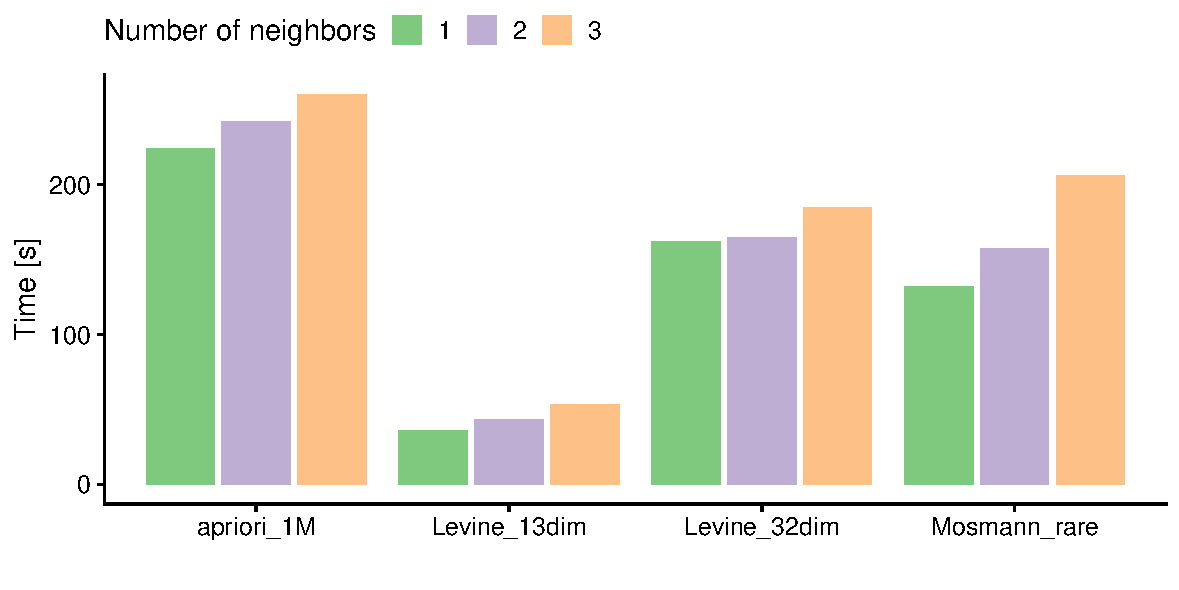
\includegraphics[width=7cm]{../img/neighbor_compare}
	\end{figure}
	
\end{frame}

\begin{frame}{Clusterings comparison}
	
	\begin{block}{Single-point dataset clusterings comparisons}
		
		\begin{columns}
			\column{\linewidth-7cm}
			
			Notable difference
			
			\column{7cm}
			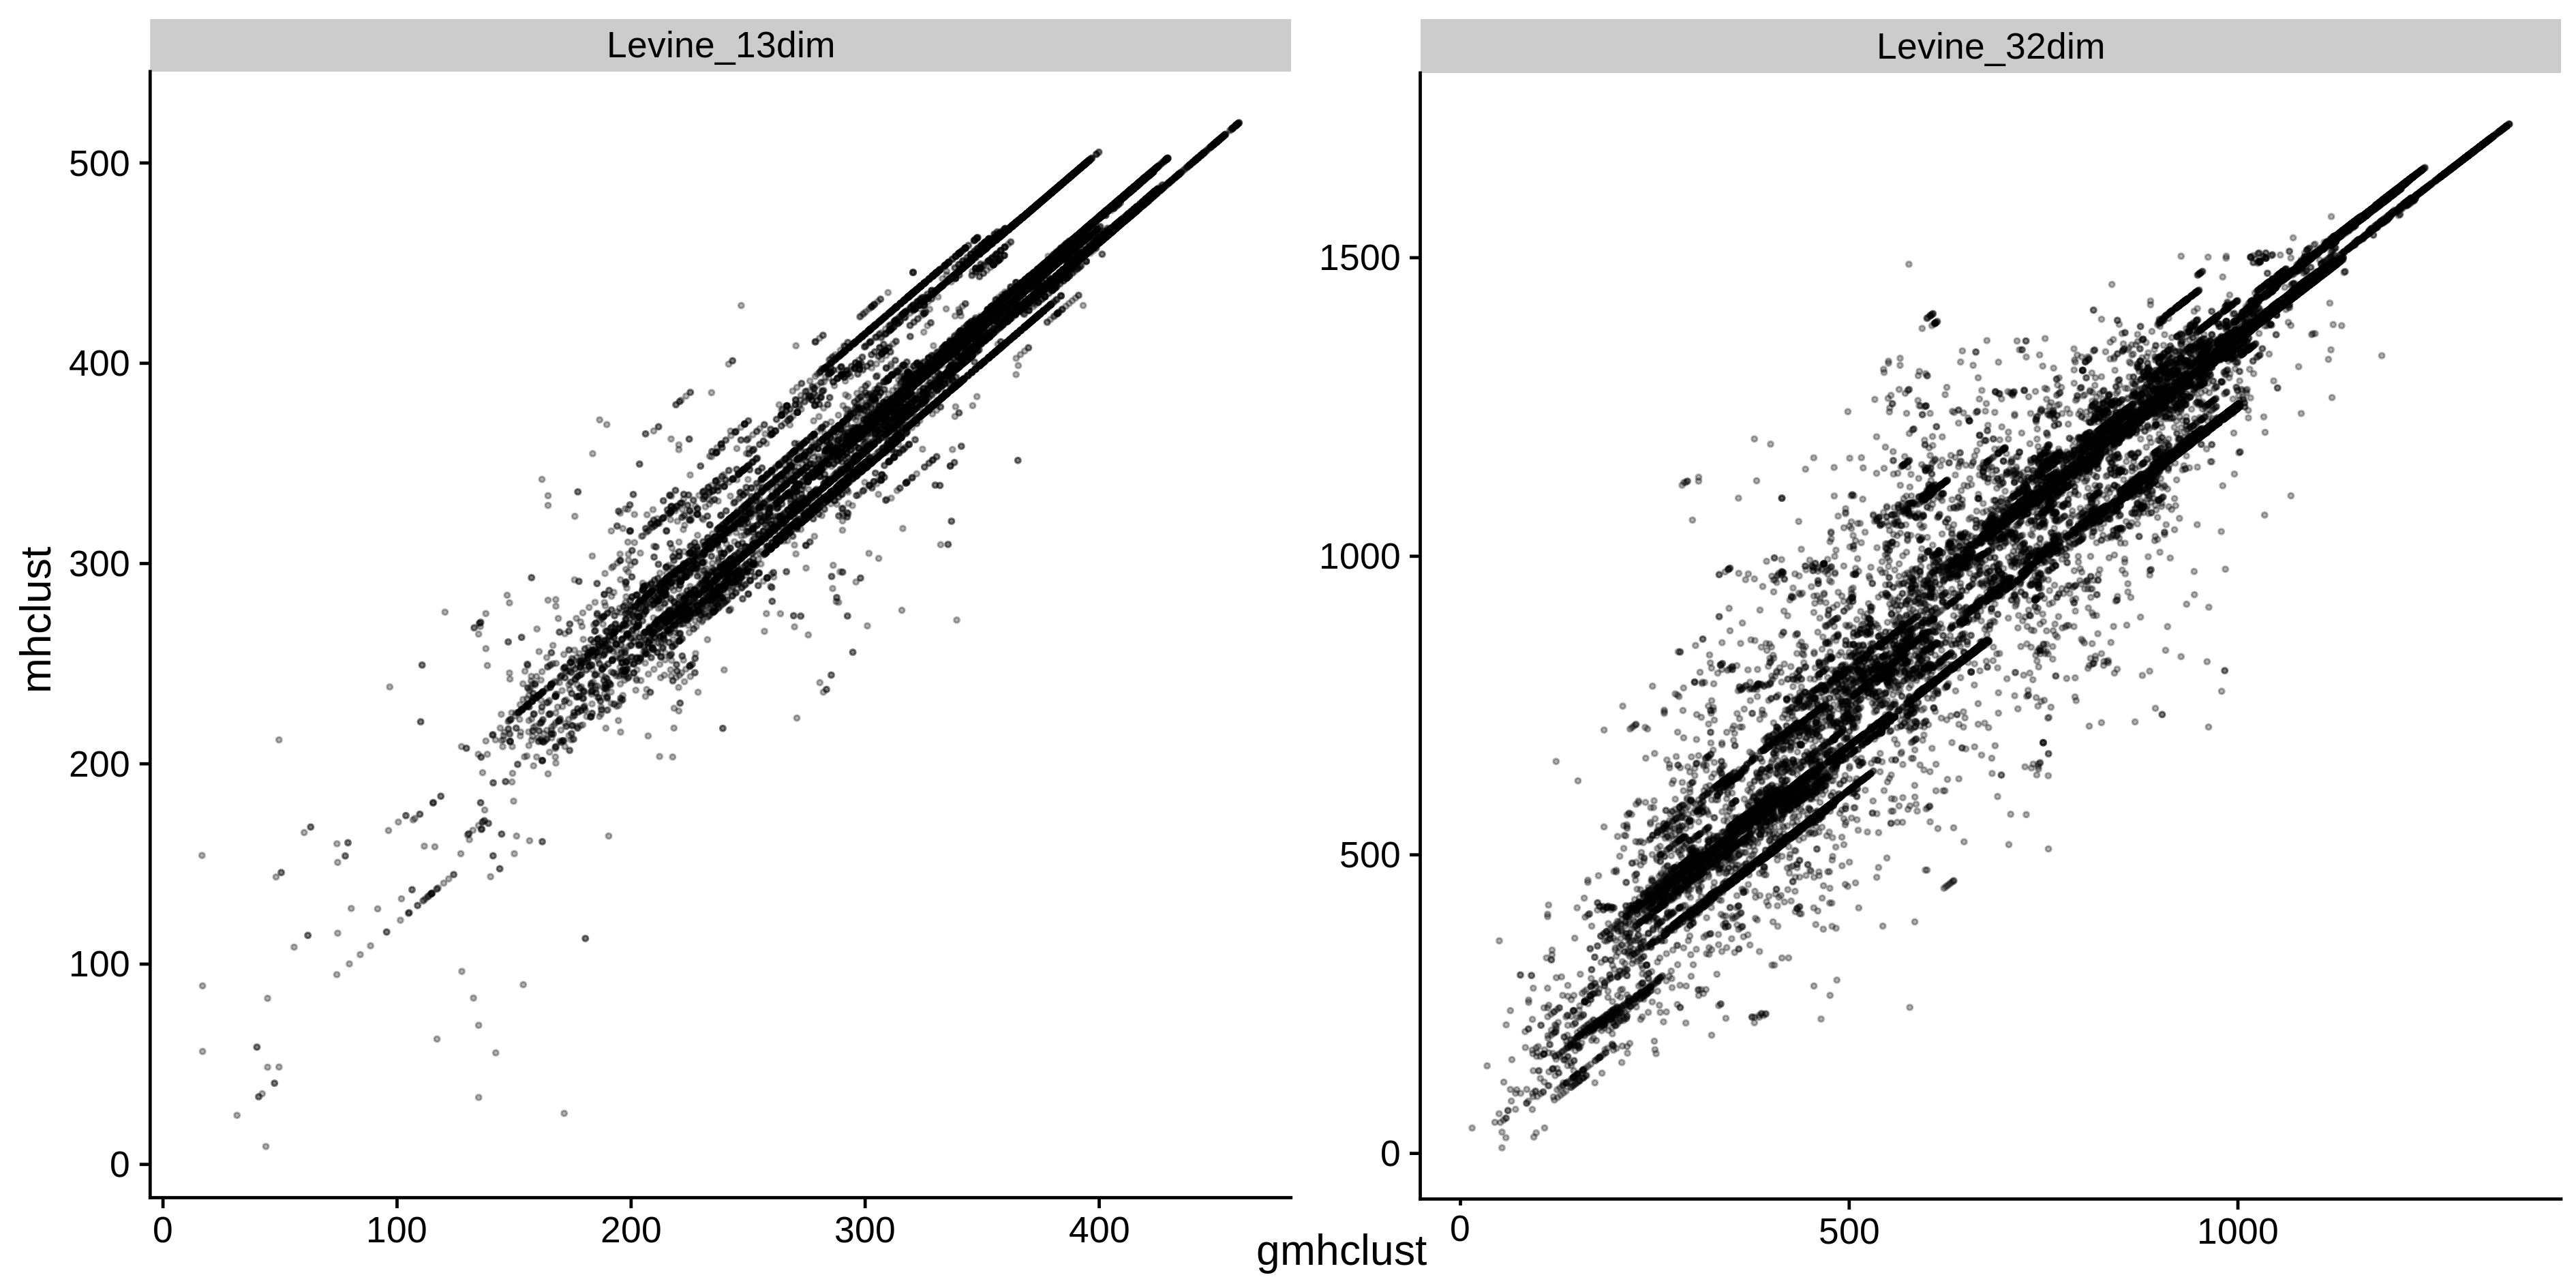
\includegraphics[width=7cm]{img/single_result}
			
		\end{columns}
	\end{block}

	\begin{block}{Apriori dataset clusterings comparisons}
		\begin{columns}
			\column{\linewidth-7cm}
			
			
			Practically no difference
			
			\column{7cm}
			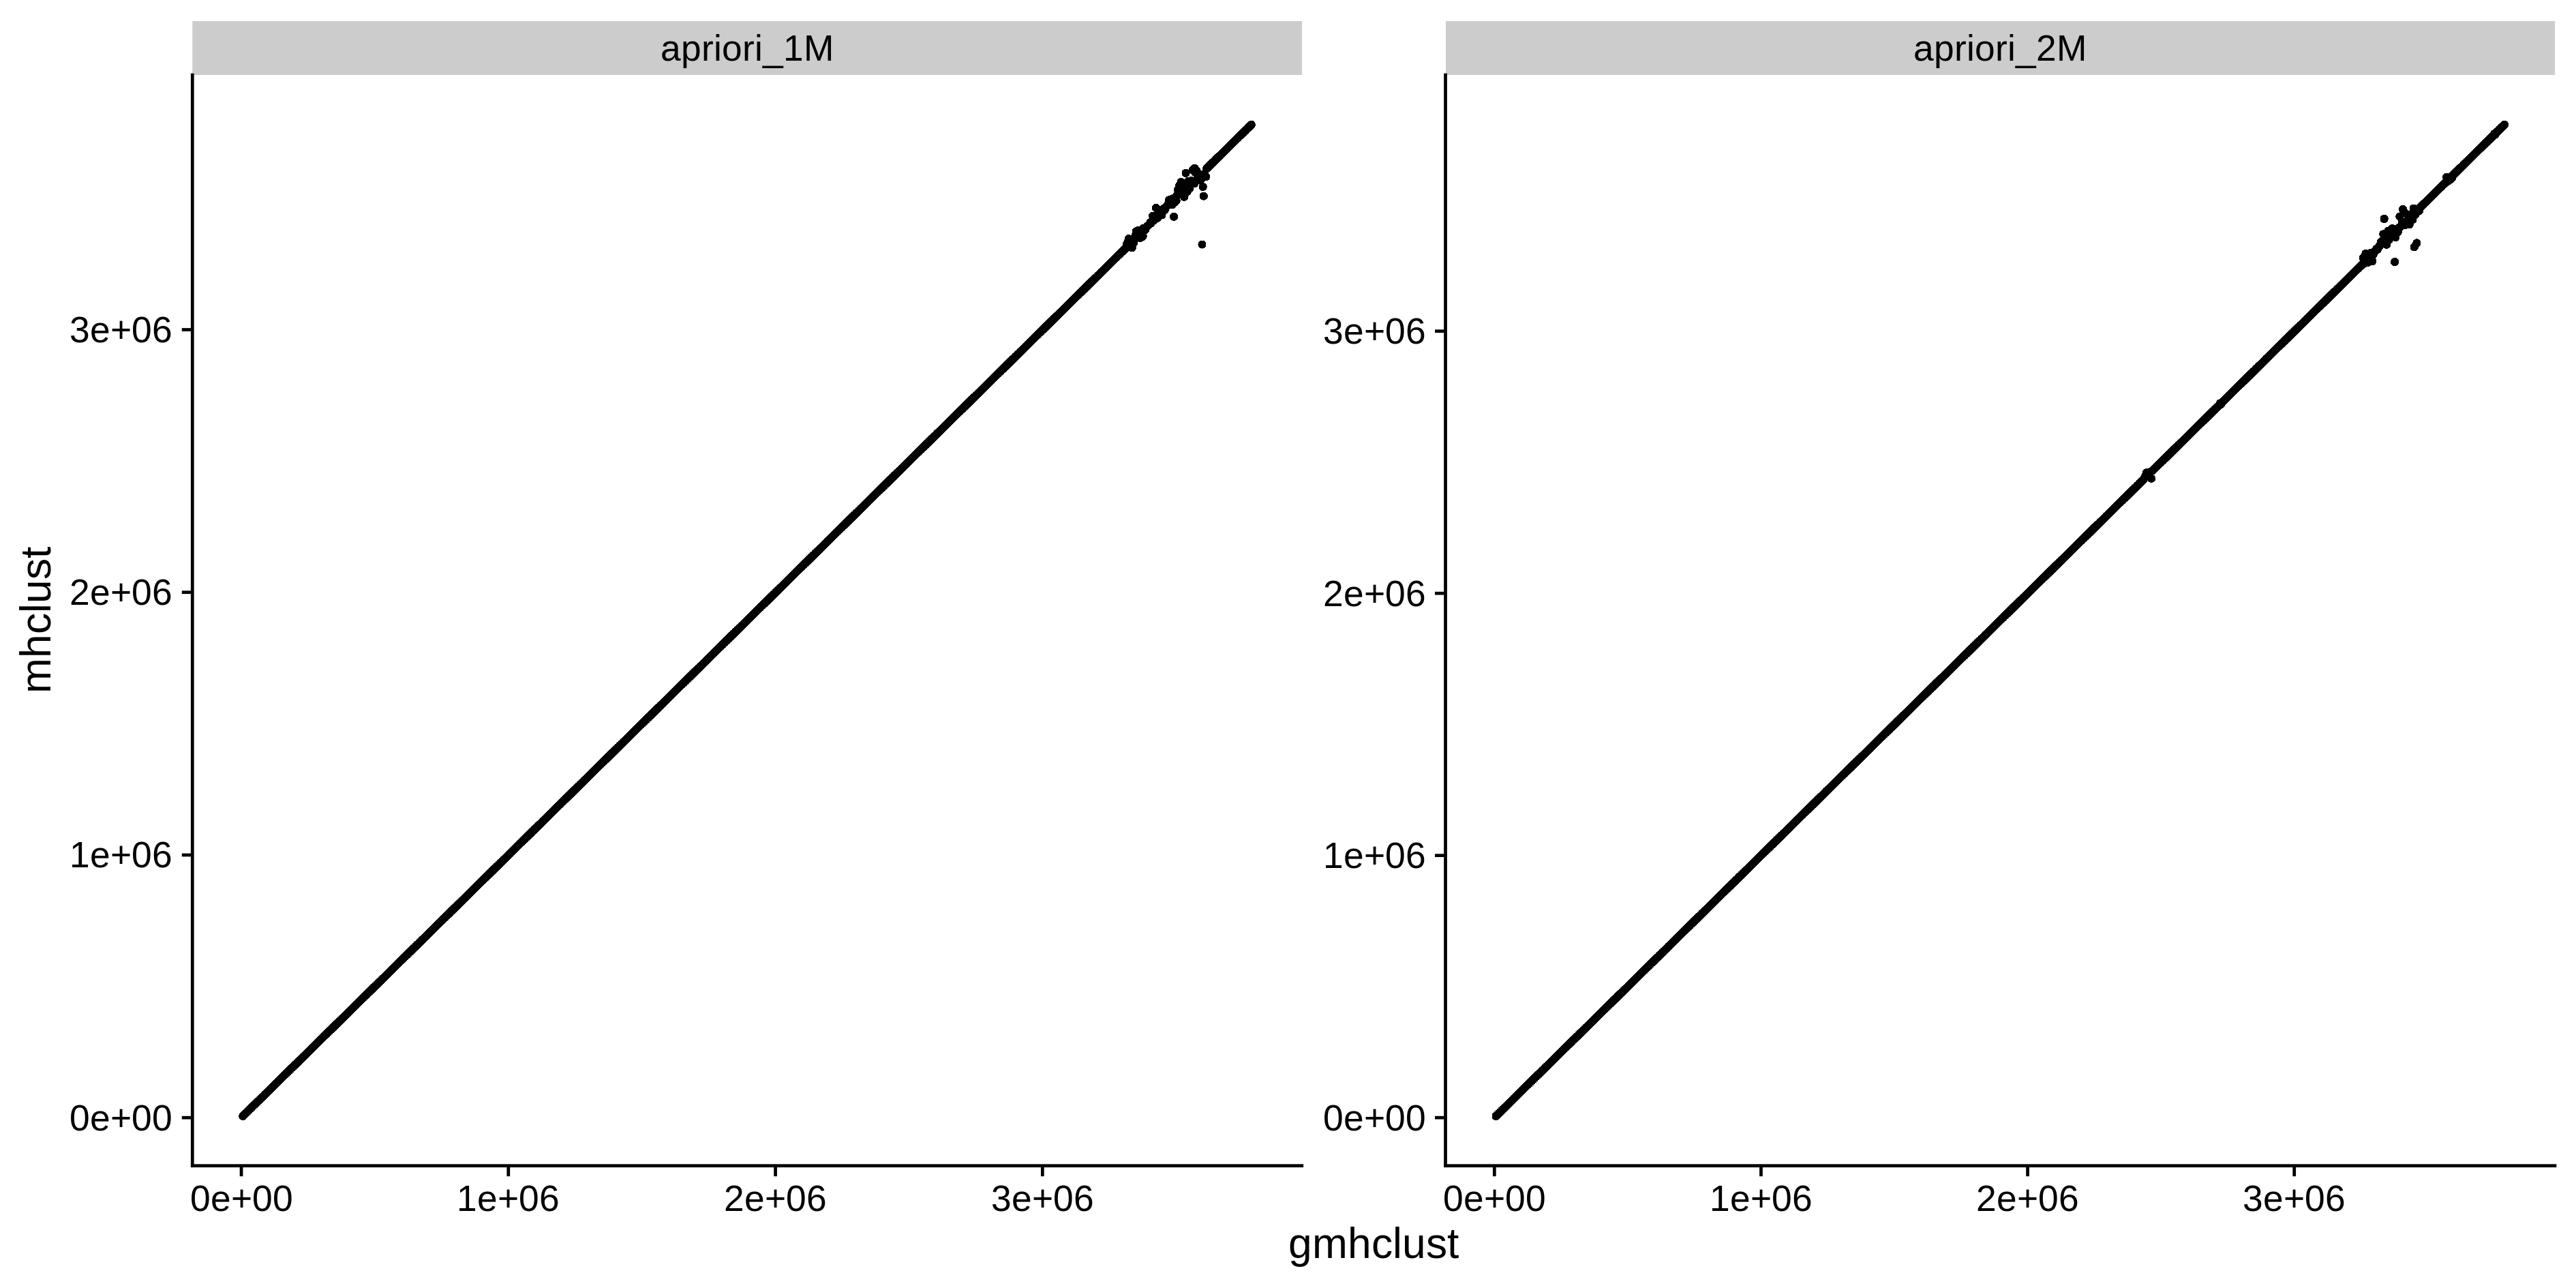
\includegraphics[width=7cm]{../img/apriori_result}
			
		\end{columns}
	\end{block}
	
\end{frame}

\begin{frame}{Conclusion}
	
	Using CUDA framework, we have implemented GPU accelerated Mahalanobis-average hierarchical clustering.
	
	We have decreased memory requirements and increased speedup of the clustering.
	
	Datasets with millions of points can be clustered efficiently. 
	
\end{frame}

\begin{frame}[standout]
  Thank you for attention.

\end{frame}


\end{document}